Передача параметров по ссылке

Оформим как процедуру вычисление $x = x div 16$

Процедура имеет один параметр-переменую x, которой в теле
процедуры присваивается новое значение. Т. е результат записывается
в некоторую ячейку памяти. И чтобы обратиться к процедуре с различными параметрами, например, a и b, ...


Процедура:

\begin{minted}{asm}
Proc_dv proc
	push CX
	mov CL, 4
	shr word ptr [BX], CL
	pop CX
	ret
Proc_dv endp
\end{minted}

Сдвиг на 4 разряда вправо эквивалентен делению нацело на шестнадцать.

При этом сохраняется содержимое регистра CX, т.к это значение перезаписывается в 4 строчке.

Т.к регистров немного, а ПП и основная программа могут использовать те же регистры, то при входе в ПП нужно сохранять все регистры, которые в этой подпрограмме используются, а перед выходом их восстанавливать. Именно для этой цели были введены команды, позволяющие сохранять все регистры общего назначения - $pusha$, $popa$, а .386 $pushad$, $popad$. Конечно, не нужно сохранять в стеке значения регистров, в которые записывается результат работы подпрограммы.

Передача параметров по ссылке в блоке параметров

Если параметров много, например, массив, адрес начала массива как блока параметров, можно передать через регистр, даже если результат ПП не будет записываться по этому адресу.

Пример:

Даны два массива целых положительных чисел без знака:
X DB 100 dup (?)
Y DB 50 dup (?)

Вычислить: DL = max(X[i]) + max(Y[I]), использовав процедуру max(A[i]), пересылая адрес массива через регистр BX,	а результат сохраняя в AL.

\begin{minted}{asm}
 lea BX, X
 mov CX, 100
 call max
 mov DL, AL
 lea BX, y
 mov CX, 50
 call max
 add DL, AL
 
 max proc
 push CX
 push BX
 mov AL, 0
 
 met1:
 cmp [BX], AL
 jle met2
 mov AL, [BX]
 
 met2:
 inc bx
 loop met1
 pop BX
 popCX
 ret
 max endp
\end{minted}

Передача параметров через стек

Этот способ передачи параметров называют универсальным, его можно использовать при любом количестве параметров, хотя он сложнее, чем передача параметров через регистры.

Если ПП имеет k параметров PP($a_1$, $a_2$ ... , $a_n$) размером в слово и параметры сохраняются в стеке в последовательности слева направо, то команды, реализующие обращение к ПП, должны быть следующими:

\begin{minted}{asm}
push a1
push a2
...
push ak
call PP
\end{minted}

В случае такого обращение содержимое стека в подпрограмме можно представить так

\begin{picture}[H]
\includegraphics{procstack.png}
\end{picture}

Обращение к параметрам в процедуре можно осуществлять с помощью значения BP, присвоив ему значение SP.

При этом мы испортим старое значение BP, которое могло быть использовано в основном программе. Поэтому следует в начале сохранить старое значение BP в стеке, а затем использовать его для доступа к параметрам, т.е тело процедуры должно начинаться следующими командами:

\begin{minted}{ssm}
PP proc near
push BP
mov BP, SP
\end{minted}

\begin{picture}[H]
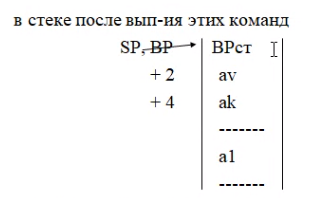
\includegraphics{procstack2.png}
\end{picture}

Для доступа к последнему параметру можно использовать выражение [BP + 4], например, mov AX, [BP + 4]; ak -> AX

После входных действий в ПП идут команды, реализующие вспомогательный алгоритм, а за ними д.б. команды, реализующие выходные действия.

\begin{minted}{asm}
pop BP
ret 2 * k
PP endp
\end{minted}

и в команде ret n - это количество освобождаемых байтов в стеке, поэтому количество д.б множено на длину параметра.

Команда ret вначале считывает значение ay, а затем удаляет из стека параметры. Очистку стека можно выполнять и не в ПП, а после выхода из нее, сразу после команды call PP, например, командой add SP, 2 * k.

Каждый способ имеет свои достоинства и недостатки.

Например, очищение в ПП позволяет сделать исполняемый код короче, а очищение в основной программе позволяет вызвать ПП несколько раз с одними и теми же параметрами последовательностями команд call.

для удобства использования параметров, переданных через стек, внутри ПП можно использовать директиву equ, чтобы при каждом обращении к параметрам не писать точное смещение относительно BP.

Пример:

push x
push y
push z
call PP

\begin{minted}{asm}
PP proc near
push BP
mov BP, SP
pp_x equ[BP + 8]
pp_y equ[BP + 6]
pp_z equ [BP + 4]

mov AX, pp_x

pop BP
ret 6
PP endp
\end{minted}

Пример передачи параметров через стек.

Пусть процедура заполняет нулями массив A[0, n - 1], а основная программа обращается к ней для обнуления массивов X[0..99] и Y[0..49]. Через стек в ПП передается имя массива и его размер, размер можно передавать по значению, а имя массива нужно передавать по ссылке, т.к этот параметр является и входным, и выходным.

\begin{minted}{asm}
zero_1 proc
push BP
mov BP. SP
push BX
push CX
mov CX, [BP + 4]
mov BX, [BP + 6]
mov byte ptr [BX], 0
inc BX
loop m1
pop CX
pop BX
pop BP
ret 4
zero_1 endp

Main:

x DB 100 dup (?)
y DB 50 dup (?)

lea AX, x
push AX
mov AX, 100
push AX
call zero_1
lea AX, y
push AX
mov AX, 50
push AX
call zero_1

end Main
\end{minted}

О передаче параметров в ПП

\begin{itemize}
\item Передача по значению
mov AX, word ptr value
\item Передача по ссылке
mov AX, offset value
call PP
\item Передача параметров по возвращаемому значению объединяет передачу по значению и по ссылке: процедура передается адрес переменной, она делает локальную копию этого параметра, работа с этой компией, а в конце процедуры записывает эту копию по переданному адресу. Этот механизм оказывается эффективным, если процедуре приходится много раз обращаться к параметру в глобальной переменной.
\item Передача параметров по результату заключатеся в том, что ПП передается адрес только для записи по этому адресму результата работы ПП.
\item Передача параметров по имени макроопределения
name macro parametr
mov AX, parametr
name endm
Обращение к ПП может быть таким:
name value
call PP
\item Передача параметров отложенным вычислением. Как и в случае передачи параметров по имени макроса, процедура получает адрес ПП, вычисляющей значение параметра. Этот механизм чаще используется в системах искусственного интеллекта и в ОС.
\end{itemize}

Использование локальных параметров.

Если локальных параметров немного, то их размещают в регистрах, но если их много, возможны различные варианты: им можно отвести место в сегменте данных, но тогда большую часть времени эта память не будет использоваться.

Лучший способ - разместить локальные переменные в стеке на время работы ПП, а после выхода из ПП их удалить. для этого после входных действий в процедуре нужно уменьшить значение указателя на вершину стека SP на количество байтов, необходимых для хранения локальных величин и затем записывать их в стек и извлекать можно с помощью выражений вида:

[BP - n], где n определяет смещение локального параметра относительно значения BP.

Например, если предполагается, что ПП будет использовать 3 локальных параметра размером в слово, то стек графически можно представить так:

\begin{picture}[H]
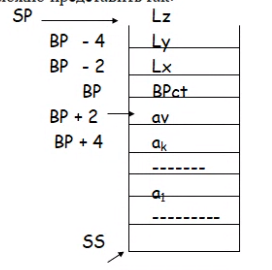
\includegraphics{procstack3.png}
\end{picture}

При выходе из процедуры перед выполнением завершающих действий нужно вернуть регистру SP его значение.

Если в стеке хранятся и фактически, и локальные параметры, то начало процедуры и её завершение должно выглядеть следующим образом:

\begin{minted}
PP proc
push BP
mov BP, SP
sub SP, k1
push AX; сохраняем в стеке регистры, используемые в ПП
----------
<тело процедуры>
-----------
pop AX ; восстанавливаем регистры
mov SP, BP; освобождаем место в стеке от локальных параметров
pop BP; восстанавливаем BP
ret k2; очищаем стек от фактических параметров
pp endp
\end{minted}

Подсчет количества различных символов в заданной строке

Строка задана как массив символов. начальный адрес ее передадим в ПП через регистр BX, длину строки через CX, а результат - через AX. Создадим процедуру, в которой выделяется 256 - байтный локальный массив L по количеству возможных символов. K - му элемент этого массива будем присваивать единицу, если символ, цифровой код которого равен К, в заданной строке существует. 

Затем подсчитаем количество единиц в этом массиве. Вначале весь массив обнуляется. К первому элементу этого массива можно обратиться так:

$L_1 = [BP - 256]$ к К - му, $L_k = [BP - 256 + k]$

Работая со строками, эту задачу можно решить проще.

\begin{minted}{asm}
count_s proc
push BP
mov BP, SP
sub SP, 256
push BX
push CX
push SI
mov AX, CX
mov CX, 256
mov SI, 0
m1:
mov byte ptr[BP - 256 + SI], 0
inc SI
loop m1

mov CX, AX
mov AX, 0
m2:
mov AL, [BX]
mov SL, AX
mov byte ptr[BP - 256 + SI], 1
inc BX
loop m2
mov AX, 0
mov CX, 256
mov SI, 0
m3:
cmp byte ptr[BP - 256 + SI], 1
jne m4
inc AX
m4:
inc SI
loop m3
pop SI
pop CX
pop BX
mov SP, BP
pop BP
ret
count_s endp
\end{minted}

Рекурсия в Ассемблере


